\documentclass[twoside]{article}%{combine}
%\usepackage{url}
\usepackage{../../tex/html}
\usepackage{amsfonts,amsmath,color,amsthm,amssymb, enumerate, bbm, subfig}
\usepackage{graphicx}
%\usepackage[DIV=14,BCOR=2mm,headinclude=true,footinclude=false]{typearea}
%\usepackage[font=small,labelfont=bf]{caption}
\usepackage{hyperref}
\usepackage{tikz, etoolbox}

\usetikzlibrary{shapes}
\usetikzlibrary{arrows}
%\usepackage[margin=1in]{geometry}
\usepackage{graphicx,amsmath,gentium,tikz,caption}
\usetikzlibrary{patterns}
\usetikzlibrary{matrix,arrows,positioning,shapes}
\usetikzlibrary{arrows.meta}
\tikzset{
  a/.style={-{Stealth[scale=1.3,angle'=45]},semithick}
}
%\usepackage{xfrac,fontspec,unicode-math}
%\setmathfont[version=cambria]{Cambria Math}
%\mathversion{cambria}
\usepackage[letterpaper, portrait, margin=1.1in]{geometry}
\usepackage{amsmath,amsthm}
\usepackage{mathtools}
\newtheorem*{definition}{Definition}
\usepackage{tcolorbox}
\tcbset{colback=white,colframe=black}
\everymath{\displaystyle}

\makeatletter
\@ifundefined{namelength}{
\newlength{\namelength}
\settowidth{\namelength}{{\bf \Large Name: }}
\newlength{\namelinelength}
\setlength{\namelinelength}{\textwidth}
\addtolength{\namelinelength}{-\namelength}
}{}

\@ifundefined{vs}{
\newcommand*{\vs}[1]{\par
  \vspace*{#1\baselineskip}%
  \@afterindentfalse
  \@afterheading
}
}{}
\makeatother



\def\fancytitle#1#2#3{
      \centerline{\framebox{\framebox{ \parbox{.8\textwidth}{ \bf ENGRI 1101 \hfill
      Engineering Applications of OR \ \ \ \  Fall 2020 \hfill #3 #1 \\
\mbox{ }\hfill
      \hfill\mbox{ } \\[1mm] \mbox{ } \hfill{\Large \bf #2}\hfill
      \mbox{ }} }}}
      
\vs 2
}

\def\handout#1#2{\fancytitle{#1}{#2}{Handout}}
\def\review#1#2{\fancytitle{#1}{#2}{Review}}
\def\homework#1#2{\fancytitle{#1}{#2}{Homework}}
\def\exercises#1{\fancytitle{}{#1}{Exercises}}
\def\solution#1#2{\fancytitle{#1}{#2}{Solutions}}
\def\final#1#2{\fancytitle{#1}{#2}{Final}
      \noindent {\bf \Large Name:} \rule{\namelinelength}{0.5pt}
      \vspace*{\baselineskip}}
\def\prelim#1#2{\fancytitle{#1}{#2}{Prelim}
      \noindent {\bf \Large Name:} \rule{\namelinelength}{0.5pt}
      \vspace*{\baselineskip}}
\def\quiz#1#2{\fancytitle{#1}{#2}{Quiz}
      \noindent {\bf \Large Name:} \rule{\namelinelength}{0.5pt}
      \vspace*{\baselineskip}}
\def\lab#1#2{\fancytitle{#1}{#2}{Lab}
      \noindent {\bf \Large Name:} \rule{\namelinelength}{0.5pt}
      \vspace*{\baselineskip}}
\def\prelab#1#2{\fancytitle{#1}{#2}{Prelab}
      \noindent {\bf \Large Name:} \rule{\namelinelength}{0.5pt}
      \vspace*{\baselineskip}}

\raggedbottom

\begin{document}

\lab{1}{The Traveling Salesman Problem}

\textbf{Objectives}
\begin{itemize}
\item   Introduce students to a real world problem solved by OR practitioners
\item   Demonstrate the use of heuristics to obtain good solutions to optimization
problems
\item  Give students an appreciation of the difficulty of solving
optimization problems exactly
\end{itemize}

\textbf{Optional Reading}
\begin{itemize}
\item
Read Handout 2 on the traveling salesman problem.
\end{itemize}
\vspace{2pt}

\subsection*{Brief description}


Finding an optimal solution to a Traveling Salesman Problem, and proving that it is, in fact, an optimal solution, is a difficult task. In practice, when a feasible solution to a difficult problem needs to be provided quickly, one often resorts to using \textbf{heuristics}, i.e., procedures for generating feasible solutions, or improving existing ones, that can be executed quickly and, hopefully, produce a pretty good result. In this lab we will consider several such heuristic procedures for the TSP.

Here are some of the heuristics we will consider for constructing a solution from scratch:
\begin{description}
\item[Nearest neighbor:] This is, perhaps the simplest procedure, which works as follows: start the tour at an arbitrary city (or point, or star, or DNA string. From now on we will call it ``city'' or ``node''.) At each step, choose the next city to go to by picking the city closest to your current location (among the cities you haven't already visited). Once all the cities have been visited, return to the first city.
\item[Nearest insertion] Start with a ``tour'' on two of the cities (e.g., the closest pair of cities).  Find new city closest to any city currently in tour. Insert the city into the tour at the best place.
\item[Farthest insertion] This algorithm is similar to the previous one: except the new city to insert is chosen as follows: for each city not already in the tour, it computes the distance to the closest node
already in the tour, and selects the node for which this
distance is \textbf{maximum} --- may seem counterintuitive, but often works very well in practice!
\end{description}
Once we have constructed a tour, we can try making some small changes to make the tour better. For instance, let us pick two edges in the current tour. Suppose we remove these edges, and add two different edges to ``reconnect'' the tour. (Notice that there is only one way to do that!) If this change improves the cost, make the change, and repeat the process on other pairs of edges, until no improvement can be made. (This only works for symmetric TSPs --- do you see why?)

The above improvement procedure is called 2-OPT. We could get more sophisticated --- removing 3 edges at a time, for example, and reconnecting the tour (this is called 3-OPT). There are even more sophisticated (fast) schemes. Notably, the Lin-Kernighan heuristics, which won't be covered, but can easily be googled.


\pagebreak

\subsection*{Part \#1: Solving the Problem Manually}

To get an appreciation for the complexity of the problem, first go to \url{http://engri1101.orie.cornell.edu/}.  Click on the \texttt{Traveling Salesman Problem} words to bring up the following image.


\begin{center}
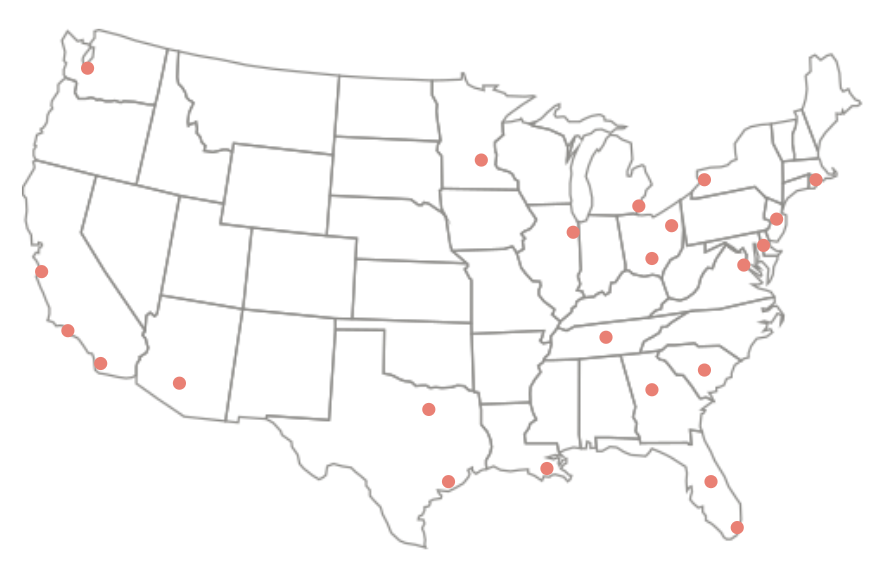
\includegraphics[width=0.8\textwidth]{BeyonceGraph.png}
\end{center}

This image shows the 23 locations where Beyonc\'{e} performed in the U.S. on her \emph{On the Run II Tour}.  Many factors would have determined where Beyonc\'{e} performed on what dates, and in turn, the order in which she visited those locations.  Let's suppose, though, that Beyonc\'{e}'s primary concern was spending as much time performing and making music as possible.  To that end, she might want to visit the 23 concert venues in the order that minimizes the total distance travelled.  

\vskip 5mm
\noindent
Try solving the TSP for this instance.  Even with 23 cities, it gets tricky!  First, draw a solution by hand on the above map.

\vskip 2in
\noindent
Now lets compute the total distance your route requires:
\begin{itemize}
\item Go back to the map on \url{http://engri1101.orie.cornell.edu/}.
\item Click any node as the `first location' of your tour.  From there, click the next city on your route.  For example, if your route has  Beyonc\'{e} go from Seattle, WA to Minneapolis, MN, you could first click Seattle and then Minneapolis.  You should see the first arc of the tour created:

\begin{center}
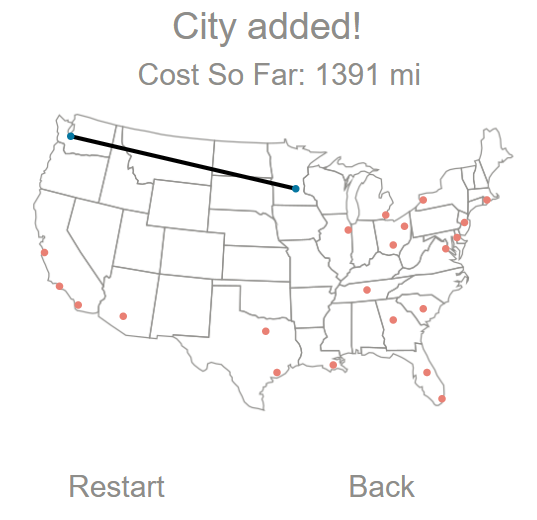
\includegraphics[width=0.5\textwidth]{BeyonceGraph2.png}
\end{center}
\item Continue successively adding cities, one at a time, in the order you drew.  If you make a mistake, hit \texttt{Back}  to remove the city you most recently added.  You can also click \texttt{Restart} to restart the entire process.
\item when you click the final 23rd location, it will automatically be connected to the first, creating a tour.  Note that, if any node is still pink, that means it has not been clicked.
\end{itemize}
What is the total distance your tour requires Beyonc\'{e} to travel?  This is reported above the map!

\vskip 2in

\subsection*{Part \#2: Heuristics for constructing tours from scratch}


In the pre-lab, you considered one particular input for the traveling
salesman problem. In the first part of the lab, you will get a feeling
for how a few different heuristics work, by running them on
the data set that you solved by hand, as well as a couple similar
instances.


You will be asked to try the first three algorithms: nearest neighbor, farthest insertion,
and nearest insertion. 

\subsubsection*{Part 2\#a: The 6 by 8 grid graph}

Back on \url{http://engri1101.orie.cornell.edu/}, click the button that says \texttt{(Next) Part 2a: 6 $\times$ 8 Grid}.  You should be brought to a 6 by 8 grid graph and will be able to select from several Heuristics.

Originally, \texttt{Mode} option should be set to Manhattan. This means that distances will be sum of vertical and horizontal distances\footnote{This is what happened in the prelab example: there is a route between any two nodes (``cities''), and the cost of that route is the sum of the vertical and horizontal ditsances separating them.  E.g. if you have to go 4 to the right and 4  up to get from node $a$ to node $b$, then the cost is $c[a, b]=3+4=7.$  The name ``Manhattan''  comes from thinking of cities with roads that form a grid.}. You can then click any of the four heuristic options listed: the latter three were explained at the beginning of the lab, while the first (\texttt{Random Neighbor}) generates a completely random tour (this is a terrible method, but useful as a baseline comparison).

First, click on \texttt{Nearest Neighbor}.  Press `d' as prompted to watch the nearest
neighbor algorithm build the tour. Although you can blithely just
hit this key over and over again, {\bf DO NOT DO SO}. For each
move, try to figure out what the algorithm does next, and then
double check by typing `d'. What sort of ``mistakes''
does the algorithm make? Note: sometimes a new edge is not easily
visible, because it lies almost completely on top of several edges
already selected for the tour. 

Once your path has exactly 3 nodes (and 2 edges), hit \texttt{Back} once, then hit `d' once (if you have already added more than 3 nodes, hit \texttt{Restart} and restart running the heuristic until you have 3 nodes).  Repeat the \texttt{Back} + `d` process several times.  You should  notice that the next node added is not always the same -- but that it is always the same distance.   Why do you think this is?  What do you think this means will happen if you run the Nearest Neighbor heuristic in full several times?


\vskip 1in

\noindent Now run the algorithm in full. Write
down the value of the solution you got. 

\vskip 1in 

\noindent Try it again. That is, click \texttt{Restart} and hit `d' to run the algorithm in full. 
Does it compute the same tour? Why do you think this is? 

\vskip 1in 
\noindent Now try running the nearest insertion
algorithm: it chooses the node closest to any node already in the
tour, and then inserts it into the tour at the best place. More
specifically, click \texttt{Nearest Insertion} on the screen, then click `d' repeatedly.  
Again, try to predict and understand how the algorithm is updating the tour in
each iteration. How does this algorithm compare? Try running two or three times.

\vskip 2in

 \noindent Another way to construct a tour is the
farthest insertion algorithm.  At each step, for each node not
already in the tour, it computes the distance to the closest node
already in the tour.  It then selects the node for which this
distance is maximum, and inserts this node into the tour in the
best place.  Click \texttt{Furthest Insertion} on the screen, then click `d' repeatedly.   How does it compare? Can you give 
any intuition why farthest insertion works well in practice?

\vskip 2in
\noindent
Compute 3 random tours using the  \texttt{Random Neighbor} button. How does the best of these compare to the
best one you computed above? Can you give some explanation for this? 

\vskip 2in 
\subsubsection*{Part 2\#b: The 9 by 9 grid graph}
\noindent Now try running all these algorithms with the larger graph grid99.  To do so, click \texttt{(Next) Part 2b: 9 $\times$ 9 Grid}.  This time, however, make sure that the  \texttt{Euclidean Distance}\footnote{The Euclidean distance between two points is their ordinary distance.  If you have to travel right 3 nodes and down 4 nodes, then the Euclidean distance is $\sqrt{3^2+4^2}=5.$} mode is selected. Does the comparison between the heuristics change?

\vskip 3 in

\subsection*{Part \#3: Heuristics for tour improvement}

Now we will try out the 2-OPT improvement algorithm.  Click \texttt{(Next) Part 3: 2-Opt}.  Follow the instructions on the web app.  You will be guided to start from a random tour and run 2-OPT one step at a time mode. Do it several times. Did you get
different results? 
\vskip 2in

Try to explain why or why not. For any data set with Euclidean distances, is it possible that an optimal tour crosses itself?
Explain why or why not. (In other words, either explain why, for any input, the
optimal tour does not cross itself, or else, give an input which
has an optimal tour that does cross itself.)

%Open grid68 again, with Manhattan distances, and generate a random
%solution. Now press `2' (then `n' repeatedly) to run the 2-OPT improvement heuristics. In each stage
%it removes two edges and include another two in order to 
%2-OPT in pause mode. In each iteration, take note of the edges that are removed
%and the edges that are being inserted. When does the heuristics finish?

%\vskip 1in \noindent
%Take 3 or 4 random tours, and run 2-OPT (in pause mode). How good
%are the tours being found?  

%\vskip 1in \noindent Compute a nearest neighbor tour and then run
%2-OPT.  Do this 3 or 4 times.   Do you think it is a better idea
%to compute a tour this way, or by starting with a random tour and
%then running 2-OPT? Why?

%\vskip 1in \noindent Now use f2 to load the input \verb|2opt2| with euclidean distance.


% \vskip 1.5in
% \noindent

% \pagebreak

% \subsection*{Part \#3: Coming up with a good tour I}

% \noindent {\bf You can do the remaining two parts of the lab in back on the original desktop.}


% You are a salesman for Stationery State, Inc., a company that specializes in
% selling stationery to state governments. In the next several months, you must
% visit the capital city of each of the lower 48 states in addition to Washington, DC. 
% You will be paid a
% fixed salary for this task no matter how long it takes you. All your expenses
% (including travel) will be out of pocket, so it is to your advantage to figure
% out the most efficient way of visiting the 49 cities. It is now your task to
% plot a tour for yourself using the attached map.  There's also an attached map (from \url{https://www.ideamia.co}) showing you state names, capital names, and state abbreviations, which might be useful in later parts of this lab.

% \begin{enumerate}
% \item   Plot the tour on the attached map.



% \vskip 1in

% \item   What methods did you use in selecting this tour? Did you just eyeball
% it or did you try to develop and apply a simple algorithm? Once you had a
% feasible route, did you try to improve upon it by changing it a little at a
% time or did you start again from scratch to try to find a better tour?


% \vskip 1in

% \item Do you think that your route is the
% best one that can be found? Why or why
% not?

% \vskip 1in

% \item  Go to course Canvas and look in the Labs folder in Files (or the lab 2 assignment)  for an EXCEL tool to compute the value of your solution (``TSP49.xls'').
% Open the spreadsheet. This spreadsheet gives very explicit directions to enter your solution.


% \end{enumerate}


% \pagebreak
% \subsection*{Part \#4: Coming up with a good tour II}

% You will now use software that is the state of the art in TSP solving, able to solve
% instances with several thousands of nodes to optimality (and prove that it is, indeed, optimal) --- Concorde.

% \vspace{5mm}
% \noindent
% Go to course Canvas and look in the Labs folder in Files (or the lab 2 assignment) for the link ``Download Concorde''. Click this link (or enter the link \url{http://www.math.uwaterloo.ca/tsp/concorde/downloads/codes/win/concorde1.1.exe} in your browser). You will need to following the instructions to install
% this software (clicking on ``run'', ``next'', ``accept'', etc.). It will install with a ``Concorde''
% icon on your desktop. Now go back to Canvas, and in the same  folder there is a ``.tsp'' file with data for the 48 capitals plus DC (listed under ``tsp49-concorde1.tsp''). Save a copy
% of this file on your ``Desktop''. Now go to your desktop and run Concorde. Under ``File'', 
% select ``Open'', and change the folder to the ``Desktop''. There you should see the data file
% that you just saved as one file listed, and select it. Now ``Solve''. What tour did this find?
% (Draw it on your map, possibly in a different color than what you used for your tour.)

% \vskip 2in

% \noindent 
% The data file that you are using was constructed by taking the latitudes and longitudes from the 
% EXCEL file, and then
% rescaling them by 1000 (to make them integers), and then computing, for each pair of cities,
% the Euclidean distance between them (that is, for two points with rescaled latitude and longitude
% coordinate $(u,v)$ and $(x,y)$, computing
% $\sqrt{(u-x)^2 + (v-y)^2}$, and then rounding that to the nearest integer). % What did this do the length of the tours computed (as compared to the length found by the EXCEL program)? (Actually, you'll probably need to think twice about what happened.) 
% Enter the tour computed by Concorde into the EXCEL program. How much better does it seem than your tour?
% \vspace{30mm}
% \pagebreak

% \includegraphics[scale=.73]{USA.png}

% \pagebreak

% \includegraphics[scale=.3, angle =-90]{USCap.png}

\end{document} 
